\documentclass[11pt,class=report,crop=false]{standalone}
\usepackage[screen]{../python}
\begin{document}

% Commande spécifique
\newcommand{\badletter}[1]{\underline{\textcolor{red}{#1}}}



%====================================================================
\chapitre{Listes I}
%====================================================================

\objectifs{Une liste est une façon de regrouper des éléments en un seul objet. Après avoir défini une liste, on peut récupérer un par un chaque élément de la liste, mais aussi en ajouter de nouveaux\ldots}


\insertvideo{Vqtmbon5_Nk}{Listes I - partie 1 - construction}

\insertvideo{pRje2HvY5OQ}{Listes I - partie 2 - manipulation}

\insertvideo{lp-MC8Hguk0}{Listes I - partie 3 - visualisation}



%%%%%%%%%%%%%%%%%%%%%%%%%%%%%%%%%%%%%%%%%%%%%%%%%%%%%%%%%%%%%%%%
%%%%%%%%%%%%%%%%%%%%%%%%%%%%%%%%%%%%%%%%%%%%%%%%%%%%%%%%%%%%%%%%

\begin{cours}[Liste (1)]

Une \defi{liste}\index{liste} est une suite d'éléments. Cela peut être une liste d'entiers, par exemple \ci{[5,-7,12,99]}, ou bien une liste de chaînes de caractères, par exemple \ci{["Mars","Avril","Mai"]} ou bien les objets peuvent être de différents types \ci{[3.14,"pi",10e-3,"x",True]}.

\begin{itemize}
  \item \textbf{Construction d'une liste.} Une liste se définit par des éléments entre crochets :
  \begin{itemize}
    \item \ci{liste1 = [5,4,3,2,1]} une liste de $5$ entiers,
    \item \ci{liste2 = ["Vendredi","Samedi","Dimanche"]} une liste de $3$ chaînes de caractères,
    \item \ci{liste3 = []} la liste vide (très utile pour la compléter plus tard  !).
  \end{itemize}

  \item \textbf{Accéder à un élément.} Pour obtenir un élément de la liste, il suffit d'écrire \ci{liste[i]} où $i$ est le rang de l'élément souhaité. 
  
  \textbf{Attention !} Le piège c'est que l'on commence à compter à partir du rang $0$ ! 
  
  Par exemple après l'instruction \ci{liste = ["A","B","C","D","E","F"]} alors  
  \begin{itemize}
    \item \ci{liste[0]} renvoie \ci{"A"}
    \item \ci{liste[1]} renvoie \ci{"B"}
    \item \ci{liste[2]} renvoie \ci{"C"}
    \item \ci{liste[3]} renvoie \ci{"D"}
    \item \ci{liste[4]} renvoie \ci{"E"}
    \item \ci{liste[5]} renvoie \ci{"F"}                   
  \end{itemize}  
  
  \medskip
  
 \myfigure{0.4}{
  \tikzinput{fig-listes-1}
}  

  
  \item \textbf{Ajouter un élément.} Pour ajouter un élément à la fin de la liste, il suffit d'utiliser la commande \ci{maliste.append(element)}\index{append@\ci{append}}\index{liste!ajouter} (\emph{to append} signifie \og{}ajouter\fg{}). 
  Par exemple si \ci{premiers = [2,3,5,7]} alors 
  \ci{premiers.append(11)} rajoute $11$ à la liste, si ensuite on exécute  la commande \ci{premiers.append(13)} alors maintenant la liste \ci{premiers} vaut \ci{[2,3,5,7,11,13]}.
  
  \item \textbf{Exemple de construction.} Voici comment construire la liste qui contient les premiers carrés :
   \begin{center}
  \begin{minipage}{0.9\textwidth}
\begin{lstlisting}
liste_carres = []          # On part d'un liste vide
for i in range(10):
    liste_carres.append(i**2)   # On ajoute un carré
\end{lstlisting}
  \end{minipage}
  \end{center}  
\`A la fin \ci{liste_carres} vaut :
\mycenterline{\ci{[0, 1, 4, 9, 16, 25, 36, 49, 64, 81]}}   
  
         
\end{itemize}
\end{cours}


\begin{cours}[Liste (2)]
\sauteligne
\begin{itemize}
  \item \textbf{Longueur d'une liste.} La longueur d'une liste est le nombre d'éléments qu'elle contient. La commande \ci{len(liste)}\index{len@\ci{len}}\index{liste!longueur} renvoie la longueur (\emph{length} en anglais). La liste \ci{[5,4,3,2,1]} est de longueur $5$, la liste \ci{["Vendredi","Samedi","Dimanche"]} de longueur $3$, la liste vide \ci{[]} de longueur $0$.
  
  \item \textbf{Parcourir une liste.} 
	Voici la façon la plus simple de parcourir une liste (et ici d'afficher chaque élément) :
\index{for@\ci{for}}\index{boucle!pour}
\begin{lstlisting}
for element in liste:
    print(element)
\end{lstlisting}

  \item \textbf{Parcourir une liste (bis).} 
  Parfois on a besoin de connaître le rang des éléments. Voici une autre façon de faire (qui affiche ici le rang et l'élément).
\begin{lstlisting}
n = len(liste)
for i in range(n):
    print(i,liste[i])
\end{lstlisting}  

\item Pour obtenir une liste à partir de \ci{range()} il faut écrire :
\mycenterline{\ci{list(range(n))}}
\end{itemize}
\end{cours}


%%%%%%%%%%%%%%%%%%%%%%%%%%%%%%%%%%%%%%%%%%%%%%%%%%%%%%%%%%%%%%%%
% Activité 1
%%%%%%%%%%%%%%%%%%%%%%%%%%%%%%%%%%%%%%%%%%%%%%%%%%%%%%%%%%%%%%%%

\begin{activite}[Intérêts simples ou composés]

\objectifs{Objectifs : créer deux listes afin de comparer deux types d'intérêts.}
\index{interets@intérêts}

\begin{enumerate}
  \item \textbf{Intérêts simples.} On dispose d'une somme $S_0$. Chaque année ce placement rapporte des intérêts en fonction de la somme initiale. 
 
  Par exemple avec une somme initiale $S_0 = 1000$ et des intérêts simples de $p = 10 \%$. Les intérêts sont de $100$. Donc au bout d'un an, je dispose d'une somme de $S_1=1100$, au bout de deux ans $S_2 = 1200$\ldots
  
  Programme une fonction \ci{interets_simples(S0,p,n)} qui renvoie les listes des sommes des $n$ premières années. Par exemple \ci{interets_simples(1000,10,3)} renvoie 
  \ci{[1000, 1100, 1200, 1300]}.
  
  
  
  \item \textbf{Intérêts composés.} Une somme $S_0$ rapporte selon des intérêts composés. Cette fois les intérêts sont calculés chaque année sur la base de la somme de l'année précédente, c'est-à-dire selon la formule : 
  $$I_{n+1} = S_n \times \frac {p}{100}$$
  
    Programme une fonction \ci{interets_composes(S0,p,n)} qui renvoie la liste des sommes des $n$ premières années. Par exemple \ci{interets_composes(1000,10,3)} renvoie 
  \ci{[1000, 1100, 1210, 1331]}.
  
  
  \item J'ai le choix entre un placement à intérêts simples de $10\%$ et un placement à intérêts composés de $7\%$.  Quelle est la solution la plus avantageuse en fonction de la durée du placement ? 
  
\end{enumerate}

\end{activite}

%%%%%%%%%%%%%%%%%%%%%%%%%%%%%%%%%%%%%%%%%%%%%%%%%%%%%%%%%%%%%%%%
%%%%%%%%%%%%%%%%%%%%%%%%%%%%%%%%%%%%%%%%%%%%%%%%%%%%%%%%%%%%%%%%

\begin{cours}[Liste (3)]
\sauteligne
\begin{itemize}
  \item \textbf{Concaténer deux listes.}\index{liste!fusionner}\index{concatenation@concaténation} Si on a deux listes, on peut les fusionner par l'opérateur \og{}\ci{+}\fg{}. Par exemple avec 
  \ci{liste1 = [4,5,6]} et \ci{liste2 = [7,8,9]}   
  \mycenterline{\ci{liste1 + liste2} \quad vaut \quad \ci{[4,5,6,7,8,9]}.}
  
    
  \item \textbf{Ajouter un élément à la fin.}\index{liste!ajouter} L'opérateur \og{}\ci{+}\fg{} fournit une autre méthode permettant d'ajouter un élément à une liste : 
  \mycenterline{\ci{liste = liste + [element]}}
  
  Par exemple \ci{[1,2,3,4] + [5]} vaut \ci{[1,2,3,4,5]}.
  Attention ! Il faut entourer l'élément à ajouter de crochets.   
  C'est une méthode alternative à \ci{liste.append(element)}.
  
  \item \textbf{Ajouter un élément au début.} Avec : 
  \mycenterline{\ci{liste = [element] + liste}}
  
  on ajoute l'élément en début de liste.
  Par exemple \ci{[5] + [1,2,3,4]} vaut \ci{[5,1,2,3,4]}. 
  
  \item \textbf{Trancher des listes.}\index{liste!sous-liste} On peut extraire d'un seul coup toute une partie de la liste : \ci{liste[a:b]} renvoie la sous-liste des éléments de rang $a$ à $b-1$.
  
  \smallskip
  
 \myfigure{0.4}{
  \tikzinput{fig-listes-3}
}    
  
    Par exemple si \ci{liste = ["A","B","C","D","E","F","G"]} alors  
  \begin{itemize}
    \item \ci{liste[1:4]} renvoie \ci{["B","C","D"]}
    \item \ci{liste[0:2]} renvoie \ci{["A","B"]}
    \item \ci{liste[4:7]} renvoie \ci{["E","F","G"]}
  \end{itemize} 
  Il faut encore une fois faire attention à ce que le rang d'une liste commence à $0$ et que le tranchage \ci{liste[a:b]} s'arrête au rang $b-1$.
  
  
\end{itemize}
\end{cours}

%%%%%%%%%%%%%%%%%%%%%%%%%%%%%%%%%%%%%%%%%%%%%%%%%%%%%%%%%%%%%%%%
% Activité 2
%%%%%%%%%%%%%%%%%%%%%%%%%%%%%%%%%%%%%%%%%%%%%%%%%%%%%%%%%%%%%%%%

\begin{activite}[Manipulation de listes]

\objectifs{Objectifs : programmer des petites routines qui manipulent des listes.}

\begin{enumerate}
  \item Programme une fonction \ci{rotation(liste)} qui décale d'un rang tous les éléments d'une liste (le dernier élément devenant le premier). La fonction renvoie une nouvelle liste.
  
  Par exemple \ci{rotation([1,2,3,4])} renvoie la liste \ci{[4,1,2,3]}.
  
  \item Programme une fonction \ci{inverser(liste)} qui inverse l'ordre des éléments d'une liste. 
  
  Par exemple \ci{inverser([1,2,3,4])} renvoie la liste \ci{[4,3,2,1]}.
  
  \item Programme une fonction \ci{supprimer_rang(liste,rang)} qui renvoie une liste formée de tous les éléments, sauf celui au rang donné. 
  
  Par exemple \ci{supprimer_rang([8,7,6,5,4],2)} renvoie la liste \ci{[8,7,5,4]} (l'élément $6$ qui était au rang $2$ est supprimé).
  
    \item Programme une fonction \ci{supprimer_element(liste,element)} renvoyant une liste qui contient tous les éléments sauf ceux égaux à l'élément spécifié. 
    
 Par exemple \ci{supprimer_element([8,7,4,6,5,4],4)} renvoie la liste \ci{[8,7,6,5]} (tous les éléments égaux à $4$ ont été supprimés).
    
\end{enumerate}

\end{activite}



\begin{cours}[Manipulation de listes]
  Tu peux maintenant utiliser les fonctions \Python{} qui font certaines de ces opérations.
  
\begin{itemize}
  \item \textbf{Inverser une liste.}\index{liste!inverser} Voici trois méthodes :\index{reverse@\ci{reverse/reversed}}
\begin{itemize}
  \item \ci{maliste.reverse()} modifie la liste sur place (c'est-à-dire que \ci{maliste} est maintenant renversée, la commande ne renvoie rien) ;
  \item \ci{list(reversed(maliste))} renvoie une nouvelle liste ;
  \item \ci{maliste[::-1]} renvoie une nouvelle liste. 
\end{itemize}  

  \item \textbf{Supprimer un élément.}  La commande \ci{liste.remove(element)}\index{liste!supprimer}\index{remove@\ci{remove}} supprime la première occurrence trouvée (la liste est modifiée). Par exemple avec \ci{liste = [2,5,3,8,5]} la commande \ci{liste.remove(5)} modifie la liste qui maintenant vaut \ci{[2,3,8,5]} (le premier $5$ a disparu).
  
   \item \textbf{Supprimer un élément (bis).}  La commande \ci{del liste[i]}\index{del@\ci{del}} supprime l'élément de rang $i$ (la liste est modifiée).
  
\end{itemize}
\end{cours}



%%%%%%%%%%%%%%%%%%%%%%%%%%%%%%%%%%%%%%%%%%%%%%%%%%%%%%%%%%%%%%%%
% Activité 3
%%%%%%%%%%%%%%%%%%%%%%%%%%%%%%%%%%%%%%%%%%%%%%%%%%%%%%%%%%%%%%%%

\begin{activite}[Tri à bulles]

\objectifs{Objectifs : ordonner une liste du plus petit au plus grand élément.}
\index{tri}

Le tri à bulles est une façon simple d'ordonner une liste, ici ce sera du plus petit au plus grand élément.
Le principe est le suivant :
\begin{itemize}
  \item On parcourt la liste en partant du début. Dès que l'on rencontre deux éléments consécutifs dans le mauvais ordre, on les échange. 
  \item À la fin du premier passage, le plus grand élément est à la fin et il ne bougera plus.
  \item On recommence du début (jusqu'à l'avant-dernier élément), cette fois les deux derniers éléments sont bien placés.
  \item On continue ainsi. Il y a en tout $n-1$ passages si la liste est de taille $n$. 
\end{itemize}

 \myfigure{0.7}{
  \tikzinput{fig-listes-2}
} 


\medskip

Voici l'algorithme du tri à bulles :
  \begin{algorithme}
  \sauteligne 
 \begin{itemize}
   \item
   \begin{itemize}
     \item Entrée : une liste $\ell$ de $n$ nombres
     \item Sortie : la liste ordonnée du plus petit au plus grand
   \end{itemize}

   \item Pour $i$ allant de $n-1$ à $0$ :\\
   \indentation Pour $j$ allant de $0$ à $i-1$ :\\
   \indentation\indentation Si $\ell[j+1] < \ell[j]$ alors échanger $\ell[j]$ et $\ell[j+1]$.
   \item Renvoyer la liste $\ell$.
 \end{itemize}  
 \end{algorithme}
 

Programme l'algorithme du tri à bulles en une fonction \ci{trier(liste)} qui renvoie la liste ordonnée des éléments. Par exemple \ci{trier([13,11,7,4,6,8,12,6])} renvoie la liste \ci{[4,6,6,7,8,11,12,13]}.

\medskip

\emph{Indications.}
\begin{itemize}
  \item Commence par définir \ci{nouv_liste = list(liste)} et travaille uniquement avec cette nouvelle liste.
  \item Pour que l'indice $i$ parcourt les indices à rebours de $n-1$ à $0$, tu peux utiliser la commande : 
\mycenterline{\ci{for i in range(n-1,-1,-1):}}

En effet \ci{range(a,b,-1)} correspond à la liste décroissante des entiers $i$ vérifiant $a \ge i > b$ (comme d'habitude la borne de droite n'est pas incluse).
\end{itemize}

\end{activite}


\begin{cours}[Tri]

Tu peux maintenant utiliser la fonction \ci{sorted()} de \Python{} qui ordonne des listes.

\index{liste!trier}
\index{sorted@\ci{sort/sorted}} 
 
  \begin{fonctionpython}[\ci{python : sorted()}]
    Usage : \ci{sorted(liste)}\\
    Entrée : une liste  \\
    Sortie : la liste ordonnée des éléments
  
  \medskip
     
   Exemple : \ci{sorted([13,11,7,4,6,8,12,6])} renvoie la liste \ci{[4,6,6,7,8,11,12,13]}.

  \end{fonctionpython}  
  
  Attention ! Il existe aussi une méthode \ci{liste.sort()} qui fonctionne un peu différemment. Cette commande ne renvoie rien, mais par contre la liste \ci{liste} est maintenant ordonnée. On parle de modification \emph{sur place}.
\end{cours}


%%%%%%%%%%%%%%%%%%%%%%%%%%%%%%%%%%%%%%%%%%%%%%%%%%%%%%%%%%%%%%%%
% Activité 4
%%%%%%%%%%%%%%%%%%%%%%%%%%%%%%%%%%%%%%%%%%%%%%%%%%%%%%%%%%%%%%%%

\begin{activite}[Arithmétique]

\objectifs{Objectifs : améliorer quelques fonctions de la fiche \og{}Arithmétique -- Boucle tant que -- I\fg{}.}

\index{facteur premier}
\index{nombre premier}

\begin{enumerate}
  \item \textbf{Facteurs premiers.}   Programme une fonction \ci{facteurs_premiers(n)} qui renvoie la liste de tous les facteurs premiers d'un entier $n\ge2$. Par exemple, pour $n = 12\,936$, dont la décomposition en facteurs premiers est $n = 2^3 \times 3 \times 7^2 \times 11$, la fonction renvoie \ci{[2, 2, 2, 3, 7, 7, 11] }.
  
  \emph{Indications.} Consulte la fiche \og{}Arithmétique -- Boucle tant que -- I\fg{}. Le corps de l'algorithme est le suivant :

\begin{center}
\begin{minipage}{0.7\textwidth}
Tant que $d \le n$:\\
\indentation Si $d$ est un diviseur de $n$, alors :\\
\indentation\indentation ajouter $d$ à la liste,\\
\indentation\indentation $n$ devient $n/d$.\\
\indentation Sinon incrémenter $d$ de $1$.
\end{minipage}
\end{center}

  \item \textbf{Liste de nombres premiers.} \'Ecris une fonction \ci{liste_premiers(n)} qui renvoie la liste de tous les nombres premiers strictement inférieurs à $n$. Par exemple \ci{liste_premiers(100)} renvoie la liste : 
  \mycenterline{\small\ci{[2,3,5,7,11,13,17,19,23,29,31,37,41,43,47,53,59,61,67,71,73,79,83,89,97]}}
  
  Pour cela, tu vas programmer un algorithme qui est une version simple du crible d'Ératosthène :
  
  \index{crible@crible d'Ératosthène}
  
  \medskip
  
   \begin{algorithme}
  \sauteligne 
 \begin{itemize}
   \item
   \begin{itemize}
     \item Entrée : un entier $n \ge 2$.
     \item Sortie : la liste des nombres premiers $< n$.
   \end{itemize}
   

  
  \item Initialiser \ci{liste} qui contient tous les entiers de $2$ à $n-1$. 
   
   \item Pour $d$ allant de $2$ à $n-1$ :\\
   \indentation Pour $k$ parcourant \ci{liste} :\\
   \indentation\indentation Si $d$ divise $k$ et $d \neq k$, alors
retirer l'élément $k$ de \ci{liste}
   \item Renvoyer \ci{liste}.
 \end{itemize}  
 \end{algorithme}
 
 %  \medskip

  \emph{Indications.}  
  \begin{itemize}
    \item Pars de \ci{liste = list(range(2,n))}.
    \item Utilise \ci{liste.remove(k)}.
   \end{itemize} 
   
   \medskip
   
  \emph{Explications.}
  Voyons comment fonctionne l'algorithme avec $n=30$.
  \begin{itemize}
    \item Au départ la liste est 
    $$[2,3,4,5,6,7,8,9,10,11,12,13,14,15,16,17,18,19,20,21,22,23,24,25,26,27,28,29]$$
    
    \item On part avec $d=2$, on élimine tous les nombres divisibles par $2$, sauf si c'est le nombre $2$ : on élimine donc $4$, $6$, $8$,\ldots, la liste est maintenant : $[2,3,5,7,9,11,13,15,17,19,21,23,25,27,29]$.
    \item On continue avec $d=3$, on élimine les multiples de $3$ (sauf $3$), après ces opérations la liste est : $[2,3,5,7,11,13,17,19,23,25,29]$.
    \item Avec $d=4$, on élimine les multiples de $4$ (mais il n'y en a plus).
    \item Avec $d=5$ on élimine les multiples de $5$ (ici on élimine juste $25$), la liste devient $[2,3,5,7,11,13,17,19,23,29]$.
    \item On continue (ici il ne se passe plus rien).
    
    \item À la fin, la liste vaut $[2,3,5,7,11,13,17,19,23,29]$.
  \end{itemize}
     
\end{enumerate}

\end{activite}



%%%%%%%%%%%%%%%%%%%%%%%%%%%%%%%%%%%%%%%%%%%%%%%%%%%%%%%%%%%%%%%%
%%%%%%%%%%%%%%%%%%%%%%%%%%%%%%%%%%%%%%%%%%%%%%%%%%%%%%%%%%%%%%%%

\begin{cours}[Visualiser une liste]

Avec le module \ci{matplotlib} il est très facile de visualiser les éléments d'une liste de nombres.

\index{matplolib@\ci{matplotlib}}
\index{module!matplolib@\ci{matplotlib}}
\index{graphique}

\begin{center}
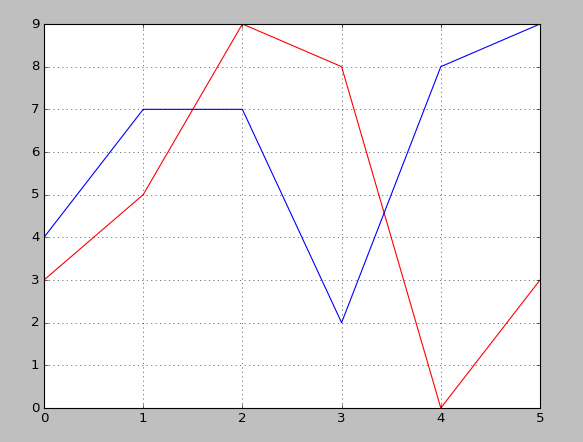
\includegraphics[scale=\myscale,scale=0.45]{ecran-liste-cours-visualisation}
\end{center}

\begin{lstlisting}
import matplotlib.pyplot as plt

liste1 = [3,5,9,8,0,3]
liste2 = [4,7,7,2,8,9]

plt.plot(liste1,color="red")
plt.plot(liste2,color="blue")
plt.grid()
plt.show()
\end{lstlisting}


\emph{Explications.}
\begin{itemize}
  \item Le module s'appelle \ci{matplotlib.pyplot} et on lui donne le nouveau nom plus simple de \ci{plt}.
  
  \item Attention ! Le module \ci{matplotlib} n'est pas toujours installé par défaut avec \Python.
  
  \item \ci{plt.plot(liste)}\index{plot@\ci{plot}} trace les points d'une liste (sous la forme $(i,\ell_i)$) qui sont reliés par des segments.
  
  \item \ci{plt.grid()} trace une grille.
  
  \item \ci{plt.show()} affiche tout.  
  
\end{itemize}

\bigskip

Pour afficher des points $(x_i,y_i)$ il faut fournir la listes des abscisses puis la listes des ordonnées :
\mycenterline{\ci{plt.plot(liste_x,liste_y,color="red")}}
Voici un exemple de graphe obtenu en affichant des points de coordonnées du type $(x,y)$ avec $y = x^2$.

\begin{center}
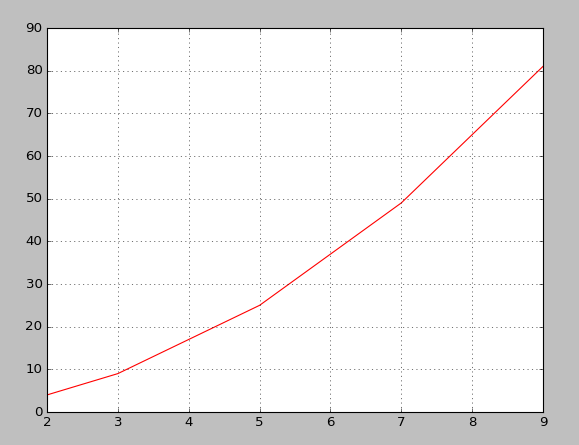
\includegraphics[scale=\myscale,scale=0.45]{ecran-liste-cours-visualisation-bis}
\end{center}


\begin{lstlisting}
import matplotlib.pyplot as plt

liste_x = [2, 3, 5, 7, 9]
liste_y = [4, 9,25,49,81]
plt.plot(liste_x,liste_y,color="red")
plt.grid()
plt.show()
\end{lstlisting}

\end{cours}


%%%%%%%%%%%%%%%%%%%%%%%%%%%%%%%%%%%%%%%%%%%%%%%%%%%%%%%%%%%%%%%%
% Activité 5
%%%%%%%%%%%%%%%%%%%%%%%%%%%%%%%%%%%%%%%%%%%%%%%%%%%%%%%%%%%%%%%%

\begin{activite}[Tir balistique]

\objectifs{Objectifs : visualiser le tir d'un boulet de canon.}

\index{tir balistique}

\begin{center}
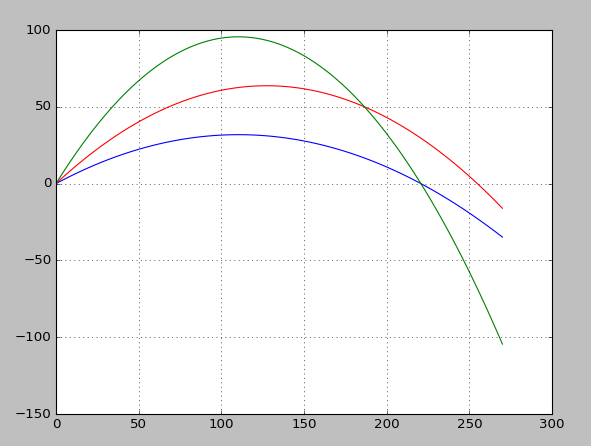
\includegraphics[scale=\myscale,scale=0.45]{ecran-liste-I-tir-bis}
\end{center}

On tire un boulet de canon depuis l'origine $(0,0)$. L'équation de la trajectoire est donnée par la formule :
$$y(x) = -\frac12  g \frac{1}{v^2 \cos^2(\alpha)} x^2 \  + \   \tan (\alpha)  x$$
où
\begin{itemize}
  \item $\alpha$ est l'angle du tir,
  \item $v$ est la vitesse initiale,
  \item $g$ est la constante de gravitation : on prendra $g = 9.81$.
\end{itemize}

\myfigure{0.7}{
  \tikzinput{fig-liste-I-tir}
} 

\begin{enumerate}
  \item Programme une fonction \ci{tir_parabolique(x,v,alpha)}
  qui renvoie la valeur $y(x)$ donnée par la formule.
  
  \emph{Indication.} Fais attention aux unités pour l'angle $\alpha$. Si par exemple tu choisis que l'unité pour l'angle soit les degrés, alors pour appliquer la formule avec \Python{} il faut d'abord convertir les angles en radians :
  $$\alpha_{\text{radians}} = \frac{2\pi}{360} \alpha_{\text{degrés}}$$
  
  \item Programme une fonction \ci{liste_trajectoire(xmax,n,v,alpha)} qui calcule la liste des ordonnées $y$ des $n+1$ points de la trajectoire dont les abscisses sont régulièrement espacées entre $0$ et $x_{\max}$. 
  
  \emph{Méthode.} Pour $i$ allant de $0$ à $n$ :
  \begin{itemize}
    \item calcule $x_i = i \cdot \frac{x_{\max}}{n}$,    
    \item calcule $y_i = y(x_i)$ par la formule de la trajectoire,
    \item ajoute $y_i$ à la liste.
  \end{itemize}  
  
  
  \item Pour $v=50$, $x_{\max} = 270$ et $n=100$, affiche différentes trajectoires selon les valeurs de l'angle $\alpha$. Quel angle $\alpha$ permet d'atteindre le point $(x,0)$ au niveau du sol le plus éloigné possible du point de tir ?
  
%  \emph{Attention !} Sur la figure affichée par \Python, les données inscrites en abscisse correspondent au rang $i$ de la suite et pas à la valeur $x$.
  
\end{enumerate}

\end{activite}


\end{document}
